\documentclass[12pt]{article}
\usepackage{amsmath}
\usepackage{graphicx}
\usepackage{hyperref}
\usepackage{listings}
\usepackage{color}
\usepackage{caption}

\title{Operating System Course Report - First Half of the Semester}
\author{A class}
\date{\today}

\begin{document}
	\maketitle
	\newpage
	
	\tableofcontents
	\newpage
	
	\section{Introduction}
	This report summarizes the topics covered during the first half of the Operating System course. It includes theoretical concepts, practical implementations, and assignments. The course focuses on the fundamentals of operating systems, including system architecture, process management, CPU scheduling, and deadlock handling.
	
	\section{Course Overview}
	\subsection{Objectives}
	The main objectives of this course are:
	\begin{itemize}
		\item To understand the basic components and architecture of a computer system.
		\item To learn process management, scheduling, and inter-process communication.
		\item To explore file systems, input/output management, and virtualization.
		\item To study the prevention and handling of deadlocks in operating systems.
	\end{itemize}
	
	\subsection{Course Structure}
	The course is divided into two halves. This report focuses on the first half, which covers:
	\begin{itemize}
		\item Basic Concepts and Components of Computer Systems
		\item System Performance and Metrics
		\item System Architecture of Computer Systems
		\item Process Description and Control
		\item Scheduling Algorithms
		\item Process Creation and Termination
		\item Introduction to Threads
		\item File Systems
		\item Input and Output Management
		\item Deadlock Introduction and Prevention
		\item User Interface Management
		\item Virtualization in Operating Systems
	\end{itemize}
	
	\section{Topics Covered}
	
	\subsection{Basic Concepts and Components of Computer Systems}
	This section explains the fundamental components that make up a computer system, including the CPU, memory, storage, and input/output devices.
	
	\subsection{System Performance and Metrics}
	This section introduces various system performance metrics used to measure the efficiency of a computer system, including throughput, response time, and utilization.
	
	\subsection{System Architecture of Computer Systems}
	Describes the architecture of modern computer systems, focusing on the interaction between hardware and the operating system.
	
	\subsection{Process Description and Control}
	Processes are a central concept in operating systems. This section covers:
	\begin{itemize}
		\item Process states and state transitions
		\item Process control block (PCB)
		\item Context switching
	\end{itemize}
	
	\subsection{Scheduling Algorithms}
	This section covers:
	\begin{itemize}
		\item First-Come, First-Served (FCFS)
		\item Shortest Job Next (SJN)
		\item Round Robin (RR)
	\end{itemize}
	It explains how these algorithms are used to allocate CPU time to processes.
	
	\subsection{Process Creation and Termination}
	Details how processes are created and terminated by the operating system, including:
	\begin{itemize}
		\item Process spawning
		\item Process termination conditions
	\end{itemize}
	
	\subsection{Introduction to Threads}
	This section introduces the concept of threads and their relation to processes, covering:
	\begin{itemize}
		\item Single-threaded vs. multi-threaded processes
		\item Benefits of multithreading
	\end{itemize}
	
	\subsection{File Systems}
	File systems provide a way for the operating system to store, retrieve, and manage data. This section explains: 
	File systems provide a way for the operating system to store, retrieve, and manage data. This section explains:
	\begin{itemize}
		\item \textit{File System Concepts}
		\item \textit{File attributes}
		\item \textit{Operations on files}
		\item \textit{File types}
		\item \textit{File structure}
		\item \textit{File access methods}
		\item \textit{Directory structure}
		
		Direktori adalah kumpulan titik yang berisi informasi tentang semua \textit{file}. Beberapa sistem menyimpan ratusan \textit{file} pada \textit{disk} ratusan \textit{gigabyte}. Untuk mengatur semua data menggunakan organisasi yang dilakukan dalam dua bagian.
		
		\begin{figure}[h!]
			\centering
			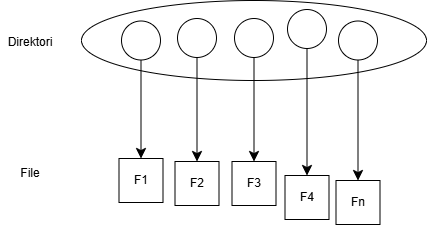
\includegraphics[width=0.8\textwidth]{aset/Halaman-1.drawio.png}
			\captionsetup{labelformat=empty}
			\caption{Gambar 8. Direktori}
		\end{figure}
		
		Pertama,\textit{ system file} dipecah ke dalam partisi, yang disebut juga “\textit{minidisc}” (pada mesin IBM) atau “volume” (pada mesin PC dan \textit{Macintosh}). Setiap disk pada sistem berisi sedikitnya satu partisi, merupakan struktur \textit{low-level} dimana \textit{file} dan direktori berada. Terkadang, partisi digunakan untuk menentukan beberapa daerah terpisah dalam satu \textit{disk}, yang diperlakukan sebagai perangkat penyimpan yang terpisah. Sistem lain menggunakan partisi yang lebih besar dari sebuah \textit{disk} untuk mengelompokkan \textit{disk} ke dalam satu struktur logika. Kedua, setiap partisi berisi informasi mengenai \textit{file }di dalamnya. Informasi ini disimpan pada\textit{ entry }dalam “\textit{device directory atau volume table of contents}”. Perangkat direktori (atau direktori) menyimpan informasi seperi nama, lokasi, ukuran dan tipe untuk semua\textit{ file} dari partisi tersebut. Organisasi \textit{file} yang umum dapat dilihat pada gambar .
		
		\begin{figure}[h!]
			\centering
			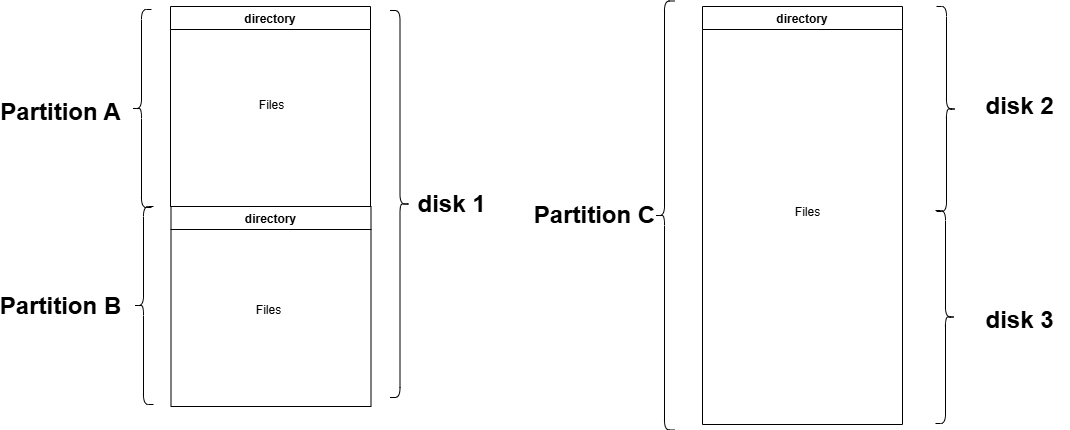
\includegraphics[width=0.8\textwidth]{aset/Halaman-2.drawio.png}
			\captionsetup{labelformat=empty}
			\caption{Gambar 9. Organisasi Sistem File}
		\end{figure}
		
		Informasi yang terdapat pada direktori adalah :  nama, tipe, alamat, panjang saat ini,  panjang maksimum, tanggal akses terakhir, tanggal perubahan terakhir, ID pemilik, informasi proteksi . Beberapa operasi yang dibentuk pada direktori adalah : Mencari \textit{file} (\textit{search}),  Membuat \textit{file} (\textit{create}), Menghapus \textit{file} (\textit{delete}), Mendaftar suatu direktori (\textit{list}), Mengubah nama \textit{file} (\textit{r\textit{ename}}),  Melintasi sistem \textit{file }(\textit{traverse})   
		Organisasi \textit{file} dan direktori disarankan yang seefisien mungkin sehingga dapat menempatkan \textit{file} dengan cepat. Selain itu dalam penamaan \textit{file} dan direktori harus nyaman untuk\textit{ user}. Dua \textit{user} dapat memberikan nama \textit{file} yang sama. \textit{File} yang sama dapat mempunyai beberapa nama. Dalam organisasi \textit{file} dan direktori juga perlu dilakukan pengelompokan \textit{file }berdasarkan \textit{property}, misalnya semua program Java, \textit{game} dan lain-lain. 
		
		\subsubsection{One - Level Directory}
		Direktori ini hanya terdiri dari satu direktori untuk setiap\textit{ user}. Pada direktori jenis ini terjadi permasalahan penamaan dan pengelompokan berdasarkan \textit{user.} 
		\begin{figure}[h!]
			\centering
			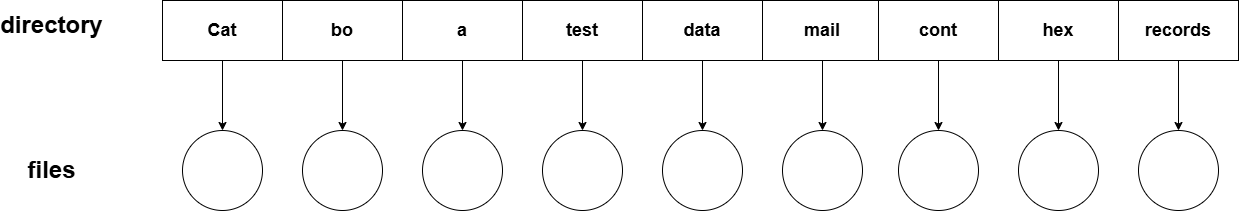
\includegraphics[width=0.8\textwidth]{aset/File system-Halaman-3.drawio.png}
			\captionsetup{labelformat=empty}
			\caption{Gambar 10.\textit{ One - Level Directory}}
		\end{figure}
		
		\subsubsection{Two - Level Directory}
		Direktori ini terdiri dari dua \textit{level} yang memisahkan direktori untuk setiap \textit{user} . Setiap \textit{file} diberi nama \textit{path}, dapat mempunyai nama \textit{file} yang sama untuk \textit{user} yang berbeda, mempunyai kapabilitas pencarian, tetapi belum dilakukan pengelompokan. 
		
		\begin{figure}[h!]
			\centering
			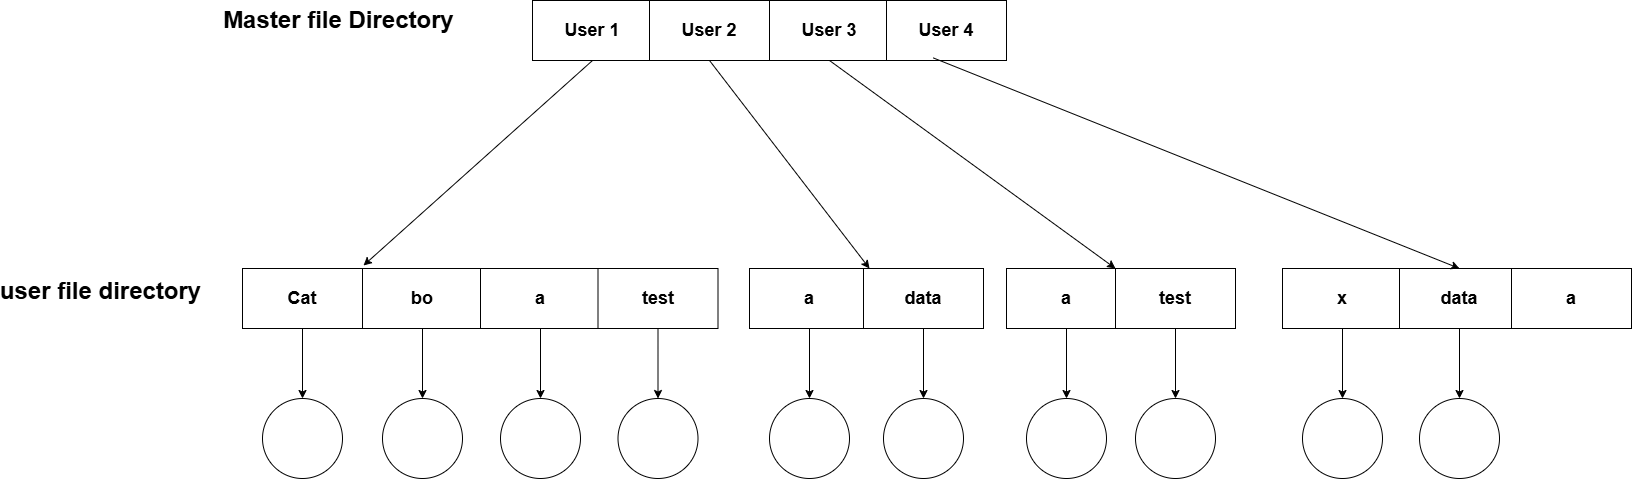
\includegraphics[width=0.8\textwidth]{aset/File system-Halaman-4.drawio.png}
			\captionsetup{labelformat=empty}
			\caption{Gambar 11. \textit{Two - Level Directory}}
		\end{figure}
		
		\subsubsection{Tree Structured Directory or Three Levels }
		Direktori berstruktur pohon merupakan struktur direktori yang biasa digunakan. Pohon mempunyai direktori \textit{root}. Setiap \textit{file }pada sistem mempunyai nama \textit{path} yang unik.
		
		\begin{figure}[h!]
			\centering
			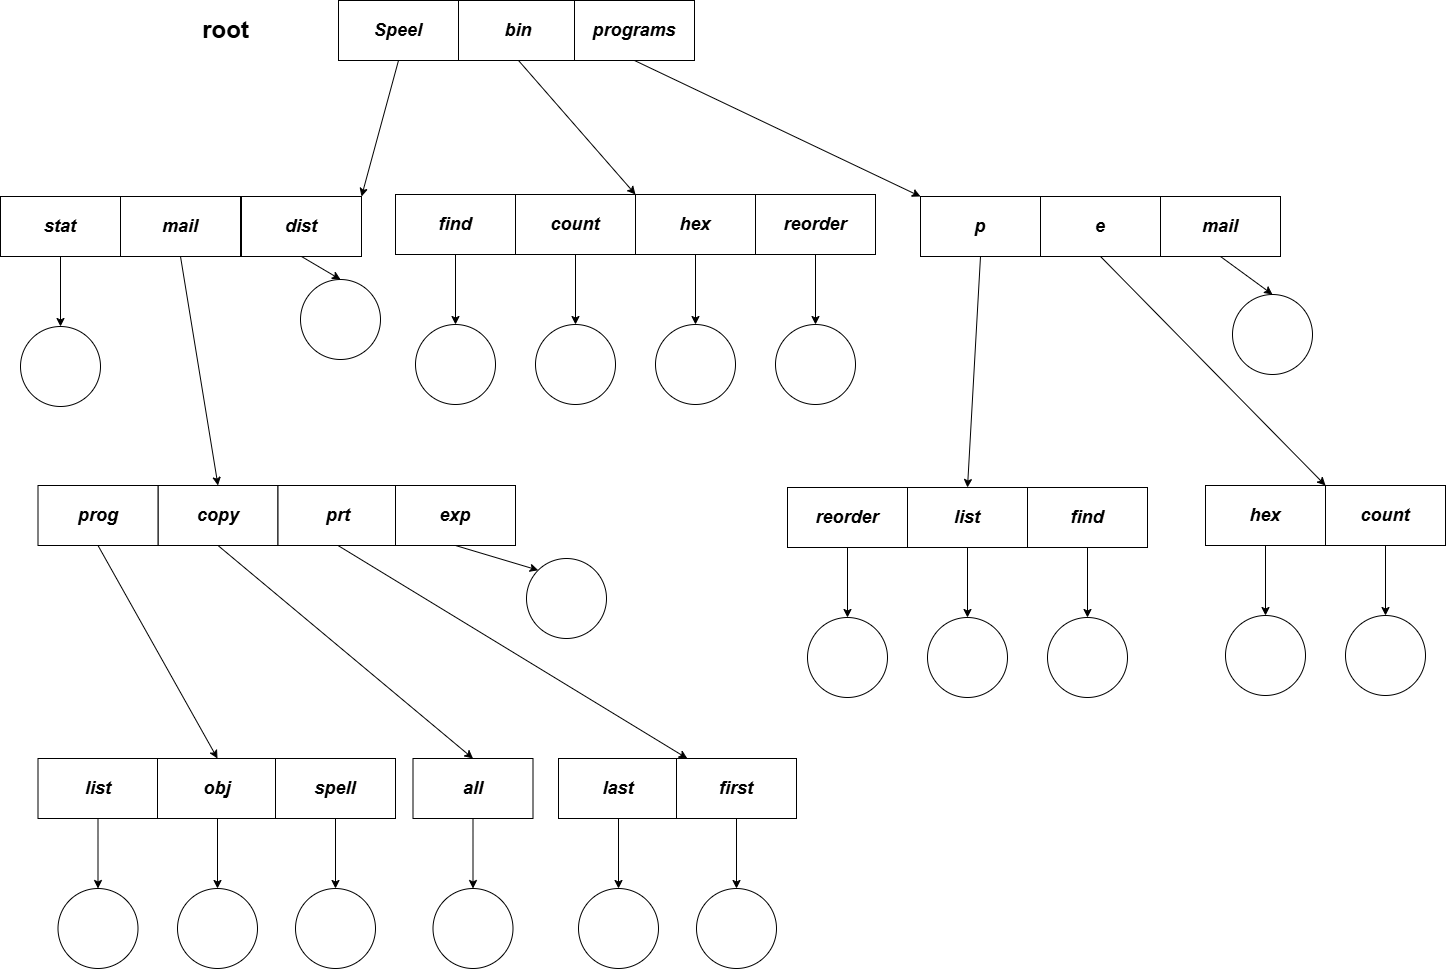
\includegraphics[width=0.5\textwidth]{aset/File system-Halaman-5.drawio.png}
			\captionsetup{labelformat=empty}
			\caption{Gambar 12.\textit{ Tree Structured Directory or Three Levels}}
		\end{figure}
		
		Pada direktori ini pencarian \textit{file} dan direktori lebih efisien, mengelompokkan \textit{file} dan dapat mengakses direktori dan sub direktori. Sebuah direktori atau sub direktori berisi kumpulan \textit{file} atau sub direktori. Sebuah direktori merupakan \textit{file} yang diperlakukan dengan cara khusus. Semua direktori mempunyai format internal yang sama. Satu bit dalam setiap masukan direktori merupakan masukan sebagai \textit{file} (0) atau sebagai sub direktori (1). \textit{Call system} khusus digunakan untuk membuat dan menghapus direktori. Nama \textit{path} dapat dibagi menjadi dua tipe yaitu nama \textit{path} “absolut” dan “relatif”. Pada saat membuat \textit{file} baru akan dilakukan pada \textit{current directory}. Demikian juga pada saat membuat direktori baru.
		
		\item \textit{file system mounting}
		\item \textit{file sharing}
		\item \textit{protection}
		\begin{thebibliography}{99}
			\bibitem{arpaci2018} 
			Silberschatz, Galvin \& Gagne. (2013). \textit{Operating System Concepts – 9th Edition}. cc.ee.ntu.edu.tw.
			\bibitem{Geeks} 
			GeeksforGeeks. (2024, Juny 24). \textit{File Systems in Operating System}. Retrieved from GeeksforGeeks: \textit{https://www.geeksforgeeks.org/file-systems-in-operating-system/}
		\end{thebibliography}
	\end{itemize}
	
	
	\subsection{Input and Output Management}
	Input and output management is key for handling the interaction between the system and external devices. This section includes:
	\begin{itemize}
		\item Device drivers
		\item I/O scheduling
	\end{itemize}
	
	\subsection{Deadlock Introduction and Prevention}
	Explores the concept of deadlocks and methods for preventing them:
	\begin{itemize}
		\item Deadlock conditions
		\item Deadlock prevention techniques
	\end{itemize}
	
	\subsection{User Interface Management}
	This section discusses the role of the operating system in managing the user interface. Topics covered include:
	\begin{itemize}
		\item Graphical User Interface (GUI)
		\item Command-Line Interface (CLI)
		\item Interaction between the user and the operating system
	\end{itemize}
	
	\subsection{Virtualization in Operating Systems}
	Virtualization allows multiple operating systems to run concurrently on a single physical machine. This section explores:
	\begin{itemize}
		\item Concept of virtualization
		\item Hypervisors and their types
		\item Benefits of virtualization in modern computing
	\end{itemize}
	
	\section{Assignments and Practical Work}
	\subsection{Assignment 1: Process Scheduling}
	Students were tasked with implementing various process scheduling algorithms (e.g., FCFS, SJN, and RR) and comparing their performance under different conditions.
	
	\subsection{Assignment 2: Deadlock Handling}
	In this assignment, students were asked to simulate different deadlock scenarios and explore various prevention methods.
	
	\subsection{Assignment 3: Multithreading and Amdahl's Law}
	This assignment involved designing a multithreading scenario to solve a computationally intensive problem. Students then applied **Amdahl's Law** to calculate the theoretical speedup of the program as the number of threads increased.
	
	\subsection{Assignment 4: Simple Command-Line Interface (CLI) for User Interface Management}
	Students were tasked with creating a simple **CLI** for user interface management. The CLI should support basic commands such as file manipulation (creating, listing, and deleting files), process management, and system status reporting.
	\subsubsection{Group 8}
	Buatlah sebuah CLI dalam Python untuk mengelola daftar tugas (\textit{to-do list}) sederhana. CLI ini harus mendukung fungsi-fungsi berikut:
	\begin{itemize}
		\item \textbf{Menambah tugas}: Pengguna bisa menambah tugas baru dengan deskripsi dan prioritas (rendah, sedang, tinggi).
		\item \textbf{Menampilkan daftar tugas}: Pengguna bisa menampilkan semua tugas yang telah ditambahkan, diurutkan berdasarkan prioritas (dari tinggi ke rendah).
		\item \textbf{Menghapus tugas}: Pengguna bisa menghapus tugas berdasarkan nomor urut yang ditampilkan.
		\item \textbf{Menandai tugas sebagai selesai}: Pengguna bisa menandai suatu tugas sebagai selesai, dan tugas tersebut akan ditampilkan dengan status "Selesai".
		\item \textbf{Keluar dari program}: Pengguna bisa keluar dari aplikasi CLI dengan mengetikkan perintah \texttt{\textbf{exit}}.
	\end{itemize}
	\textbf{jawaban :}
	
	\lstset{ 
		language=Python,
		backgroundcolor=\color{white}, 
		keywordstyle=\color{blue},
		basicstyle=\ttfamily\footnotesize, 
		breaklines=true,  
		frame=single, 
		showstringspaces=false, 
	}
	
	\begin{lstlisting}
		class ToDoListCLI:
		def __init__(self):
		self.tasks = []
		
		def add_task(self, description, priority):
		"""Menambahkan tugas baru dengan deskripsi dan prioritas."""
		task = {
			'description': description,
			'priority': priority,
			'status': 'Belum selesai'
		}
		self.tasks.append(task)
		print(f"Tugas '{description}' dengan prioritas '{priority}' berhasil ditambahkan.")
		
		def list_tasks(self):
		"""Menampilkan daftar tugas yang diurutkan berdasarkan prioritas."""
		if not self.tasks:
		print("Tidak ada tugas dalam daftar.")
		else:
		# Urutkan tugas berdasarkan prioritas (tinggi -> rendah)
		sorted_tasks = sorted(self.tasks, key=lambda x: x['priority'], reverse=True)
		print("\nDaftar Tugas:")
		for idx, task in enumerate(sorted_tasks, 1):
		print(f"{idx}. [{task['status']}] {task['description']} (Prioritas: {task['priority']})")
		
		def delete_task(self, task_number):
		"""Menghapus tugas berdasarkan nomor urut."""
		if 0 < task_number <= len(self.tasks):
		removed_task = self.tasks.pop(task_number - 1)
		print(f"Tugas '{removed_task['description']}' berhasil dihapus.")
		else:
		print("Nomor tugas tidak valid!")
		
		def mark_task_complete(self, task_number):
		"""Menandai tugas sebagai selesai."""
		if 0 < task_number <= len(self.tasks):
		self.tasks[task_number - 1]['status'] = 'Selesai'
		print(f"Tugas nomor {task_number} berhasil ditandai sebagai selesai.")
		else:
		print("Nomor tugas tidak valid!")
		
		def cli(self):
		"""Command Line Interface untuk To-Do List."""
		print("Selamat datang di To-Do List CLI!")
		while True:
		command = input("\nMasukkan perintah (add/list/delete/complete/exit): ").lower()
		
		if command == 'add':
		description = input("Masukkan deskripsi tugas: ")
		priority = input("Masukkan prioritas (tinggi/sedang/rendah): ").lower()
		if priority in ['tinggi', 'sedang', 'rendah']:
		self.add_task(description, priority)
		else:
		print("Prioritas tidak valid! Masukkan salah satu: tinggi, sedang, atau rendah.")
		
		elif command == 'list':
		self.list_tasks()
		
		elif command == 'delete':
		self.list_tasks()
		try:
		task_number = int(input("Masukkan nomor tugas yang akan dihapus: "))
		self.delete_task(task_number)
		except ValueError:
		print("Input harus berupa angka!")
		
		elif command == 'complete':
		self.list_tasks()
		try:
		task_number = int(input("Masukkan nomor tugas yang akan ditandai sebagai selesai: "))
		self.mark_task_complete(task_number)
		except ValueError:
		print("Input harus berupa angka!")
		
		elif command == 'exit':
		print("Keluar dari To-Do List CLI...")
		break
		
		else:
		print("Perintah tidak valid! Silakan coba lagi.")
		
		todo_cli = ToDoListCLI()
		todo_cli.cli()
		
	\end{lstlisting}
	\subsection{Assignment 5: File System Access}
	In this assignment, students implemented file system access routines, including:
	
	\begin{itemize}
		\item File creation and deletion
		\item Reading from and writing to files
		\item Navigating directories and managing file permissions
	\end{itemize}
	
	\section{Conclusion}
	The first half of the course introduced core operating system concepts, including process management, scheduling, multithreading, and file system access. These topics provided a foundation for more advanced topics to be covered in the second half of the course.
	
\end{document}